
%(BEGIN_QUESTION)
% Copyright 2010, Tony R. Kuphaldt, released under the Creative Commons Attribution License (v 1.0)
% This means you may do almost anything with this work of mine, so long as you give me proper credit

Calculate the maximum amount of current allowed through a 185 mH inductor to limit the energy stored in that inductor to a maximum of 40 mJ.

\vskip 10pt

$I_{max}$ = \underbar{\hskip 50pt} mA

\vskip 10pt

Next, calculate the necessary resistor value to ensure the circuit current never exceeds this maximum limit, assuming the inductor has a coil resistance of 15 $\Omega$:

$$\includegraphics[width=15.5cm]{i04736x01.eps}$$

$R$ = \underbar{\hskip 50pt} $\Omega$

\underbar{file i04736}
%(END_QUESTION)





%(BEGIN_ANSWER)

$I_{max}$ = \underbar{\bf 657.6} mA

\vskip 10pt

$R$ = \underbar{\bf 21.497} $\Omega$

%(END_ANSWER)





%(BEGIN_NOTES)

{\bf This question is intended for exams only and not worksheets!}

%(END_NOTES)


